\section {Introduction}

Many of the searches for \charginopm and \neutralinotwo in ATLAS \cite{Aad:2012hba, ATLAS:2012ab} and CMS \cite{Chatrchyan:2012mea} involves the search for signal events with 3 leptons and \met. On the other hand there are very few searches involving final states with $\tau$ leptons due to the the larger $\tau$ misidentification rate which makes harder to keep the background under control as well as having low \pt thresholds for triggering.

There is however the possibility to study final states with $2\tau$ and \met coming from the decay of \charginopm and \neutralinotwo produced by Vector Boson Fusion (VBF) processes. This search comes with some important advantages.

Firstly with the increasing LHC luminosity both ATLAS and CMS needs to raise the \pt thresholds on the triggered objects. Is it possible however to probe signal for SUSY in VBF events by triggering over the VBF properties of the event, leaving the decay products of \charginopm and \neutralinotwo free from trigger bias. 

Secondly scenarios involving the naturalness of SUSY allows \stau lighter than \smuon and \selectron for high values of \tanbeta. A light \stau with small mass splitting also is favored in coannihilation processes \cite{Griest:1990kh} that set the relic density to correct values, in the case of Bino dark matter. Light \stau is also motivated in the context of the MSSM by the enhancement of the $H \longrightarrow \gamma\gamma$ channel \cite{Carena:2011aa}. All of these facts stress on the importance of the search for low \pt $\tau$ final states with large background contribution, for which production by the VBF processes since is possible to take advantage of its signature in order to reduce the background contribution. 

As third and final reason a VBF based searches are complementary to the existing one at LHC based on Drell-Yan production since is not constrained by any trigger bias. 

\begin{figure}[tbh!]
	\centering
	\begin{tabular}{cc}
		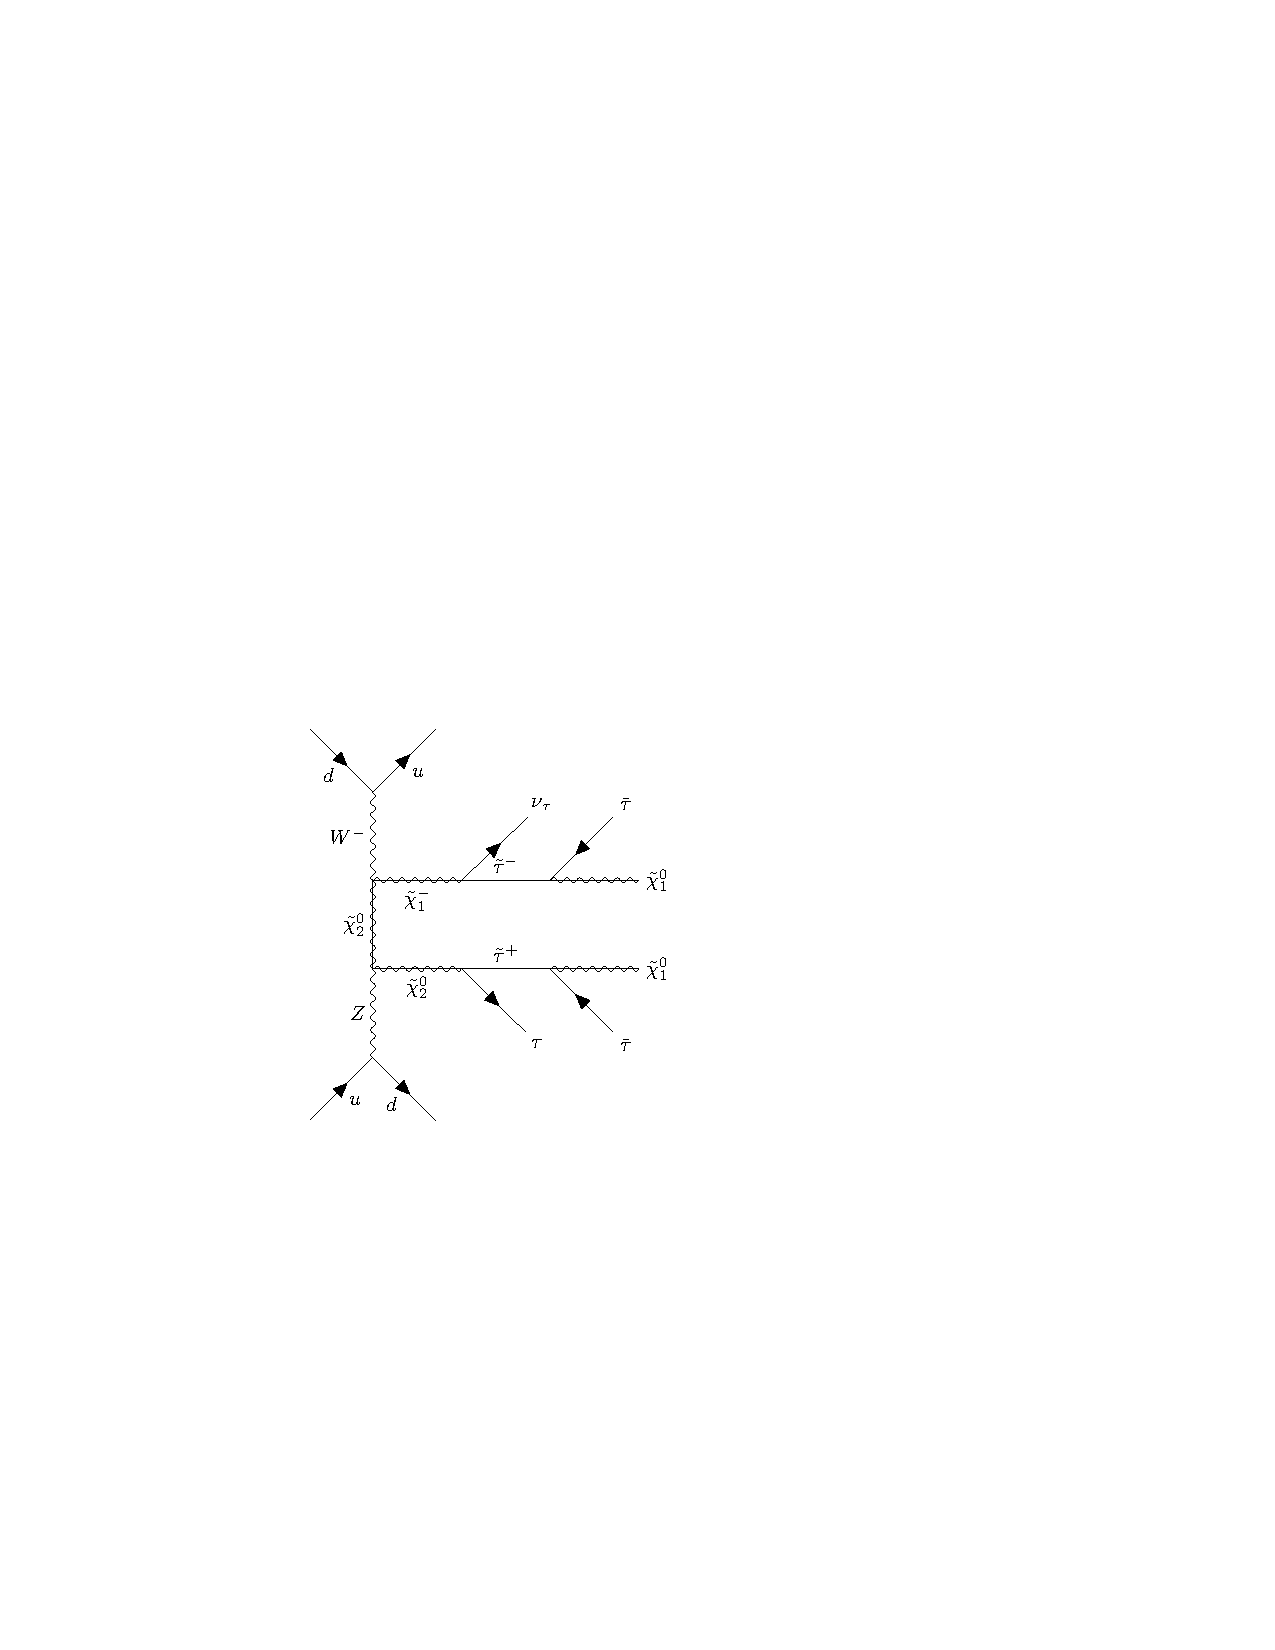
\includegraphics[width=0.48\textwidth]{diagrams/pics/signal_C1N2.pdf}
		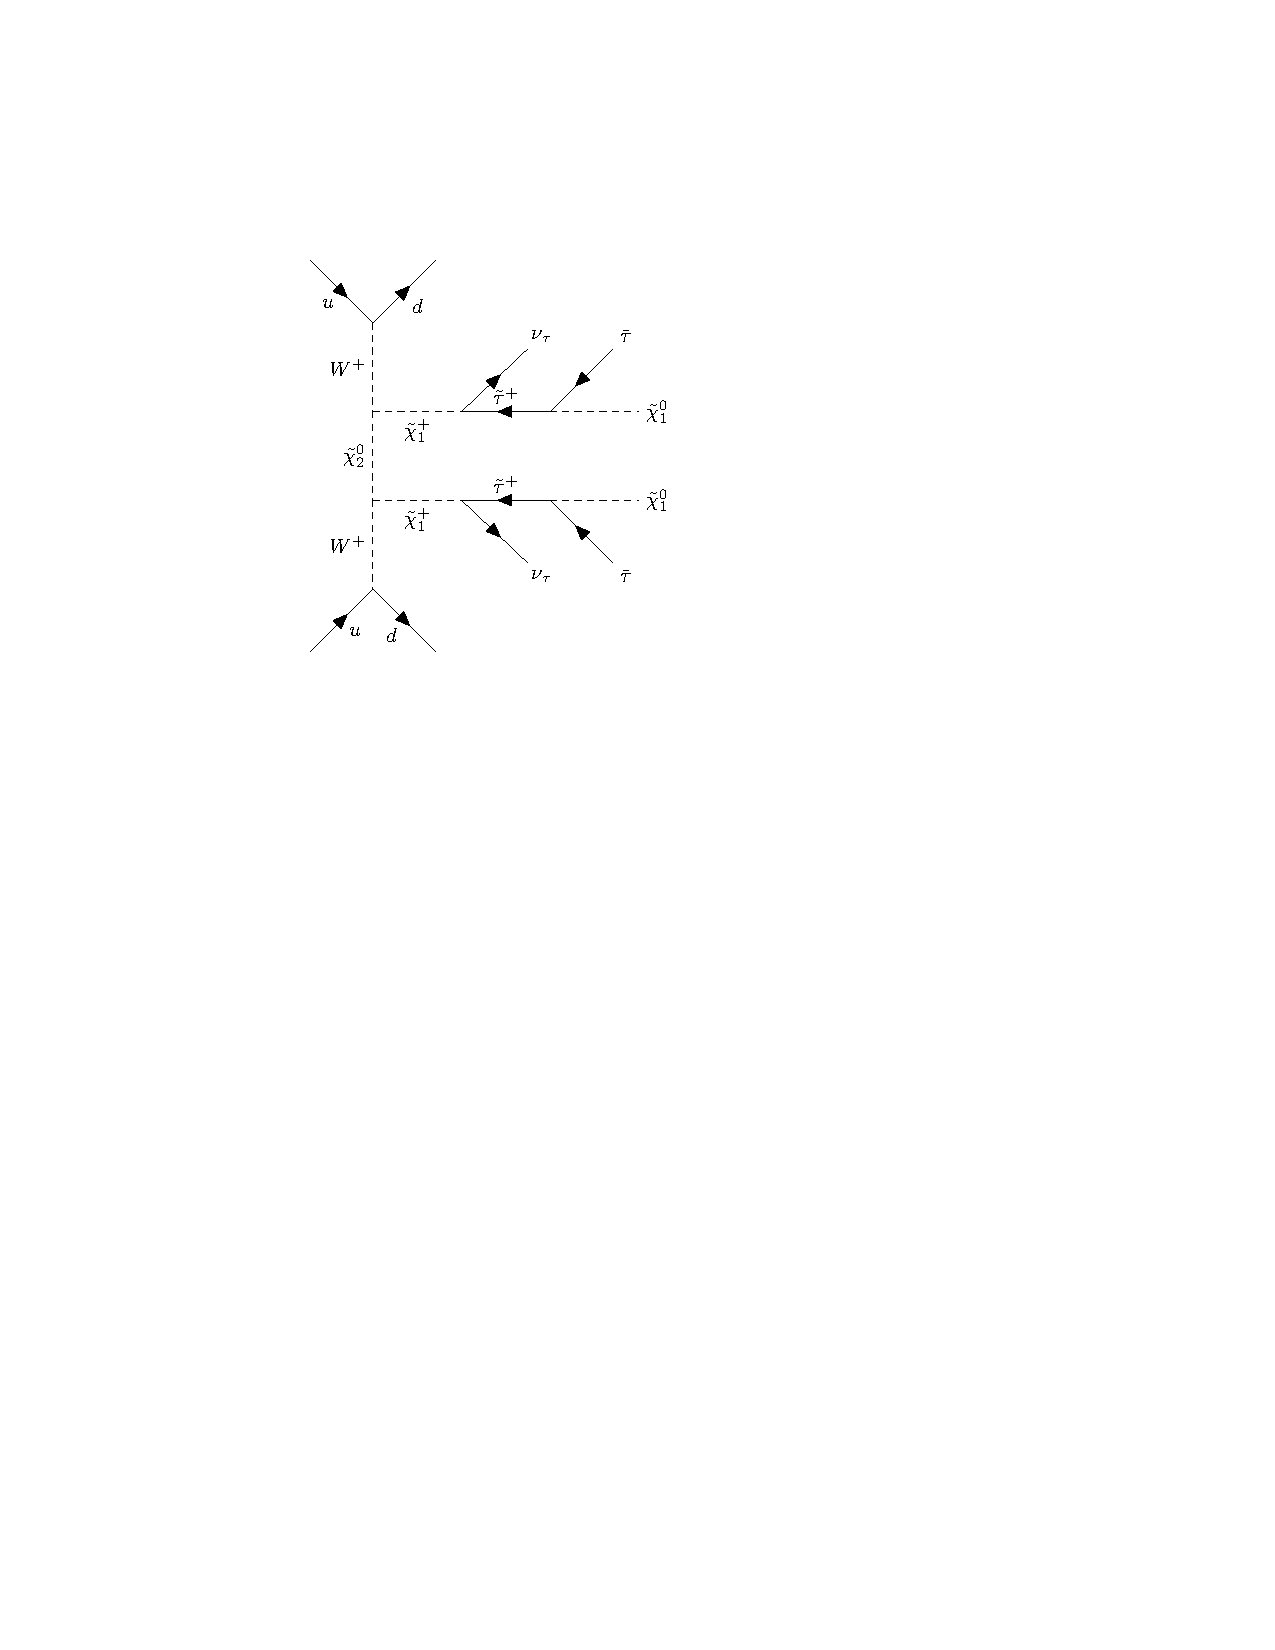
\includegraphics[width=0.48\textwidth]{diagrams/pics/signal_C1C1.pdf} 		
	\end{tabular}
	\caption{Diagrams of (left) \charginopm \neutralinotwo and (right) \charginopm \charginomp pair production through vector-boson fusion followed by their decays to $\tau$ leptons and the LSP.}
	\label{fig:VBF_diagrams}
\end{figure}

The Feynman diagrams for the typical \charginopm \neutralinotwo pair production are shown on  Figure \ref{fig:VBF_diagrams}. The \charginopm and \neutralinotwo coming from the VBF processes decays into the multiple leptons and \neutralinoone final state with the following decay process for \charginopm

\begin{equation}
\charginopm \longrightarrow \stau^{\pm} \nu \longrightarrow \neutralinoone \tau^{\pm} \nu
\end{equation}

and similarly for \neutralinotwo

\begin{equation}
\neutralinotwo \longrightarrow \stau^{\pm} \tau^{\mp} \longrightarrow \neutralinoone \tau \tau
\end{equation}

\section {Search Strategy}
\label{section::search_strategy}

For this type of search several benchmark points are defined under the following constraints:
\begin{itemize}
	\item The \charginopm and \neutralinotwo are mainly Wino-like, while the \neutralinoone is mainly Bino-like;
	\item The \charginomp mass similar to the \neutralinotwo mass ($m_{\charginopm} \sim m_{\neutralinotwo}$) and with values of 100, 200 and 300 \gev;
	\item The mass gap between the \stau and \charginopm is either 5 \gev or $(m_{\stau} - m_{\charginopm})/2$;
	\item The LSP mass is either $\neutralinoone = 0$, or 50 \gev;
\end{itemize}

The processes taken into account are

\begin{equation}
pp \longrightarrow \charginopm \charginomp jj, \quad pp \longrightarrow \charginopm \neutralinotwo jj, \quad pp \longrightarrow \neutralinotwo \neutralinotwo jj
\end{equation}

\begin{figure}[tbh!]
	\centering
	\begin{tabular}{cc}
		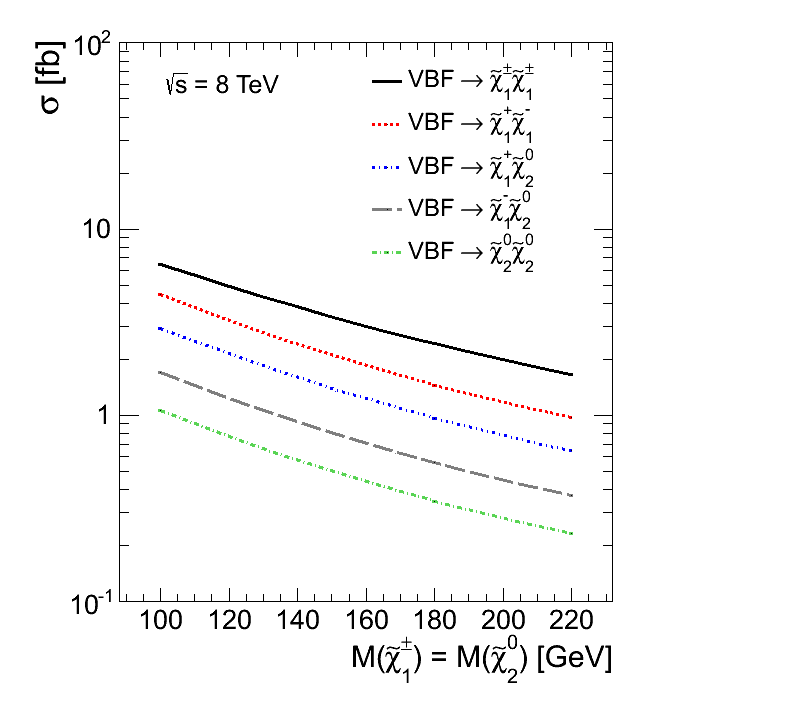
\includegraphics[width=0.75\textwidth]{analysis/pics/VBFXsection.png}
	\end{tabular}
	\caption{VBF production cross-section at \CM = 8 \tev as a function of mass for various channels after imposing \ensuremath{\deltaeta > 4.2} using Madgraph 4 \cite{Dutta:2012xe}.}
	\label{fig:VBF_xsec}
\end{figure}

The cross-section prediction for those processes are summarized in Figure \ref{fig:VBF_xsec} as function of the \charginomp - \neutralinotwo mass.

The search strategy can be divided in two distinct parts: the first one considers the kinematic of the jets produced via VBF in order to reduce the contribution coming  from V + jets events (where V is ether the W or Z boson); the second one takes into account the properties of the supersymmetric particles falling into the inner region of the detector (centrally produced) in order to reduce the all the non-supersymmetric background contributions.

The main feature of VBF processes is the production of two jets aimed at the forward-backward region of the detector with high \pt and large \deltaeta. By adding to the event selection the requirements on the di-jet \deltaeta as well as the di-jet invariant mass \ensuremath{m_{j_{1}j_{2}}} the background contribution coming from V+jets and \ttbar events is kept under control. In order to generate super-symmetric particles, the incoming partons need to have an high momentum, therefore the leading jet from the VBF-produced di-jet pair is expected to have high \pt. The addition of a \pt cut on leading jets keeps further reduces background contributions. Figure \ref{fig:VBF_mjj_ptj1} shows a study on \ensuremath{m_{j_{1}j_{2}}} and leading jet \pt distributions for \charginopm \charginopm pair production by VBF processes, V+jets background, and VV background produced by VBF processes for \ensuremath{m_{\charginopm} = m_{\neutralinotwo} = 300\gev}, \ensuremath{m_{\charginopm} - m_{\tilde{\tau}} = 5\gev} and \ensuremath{m_{\neutralinoone} = 0\gev}.

\begin{figure}[tbh!]
	\centering
	\begin{tabular}{cc}
		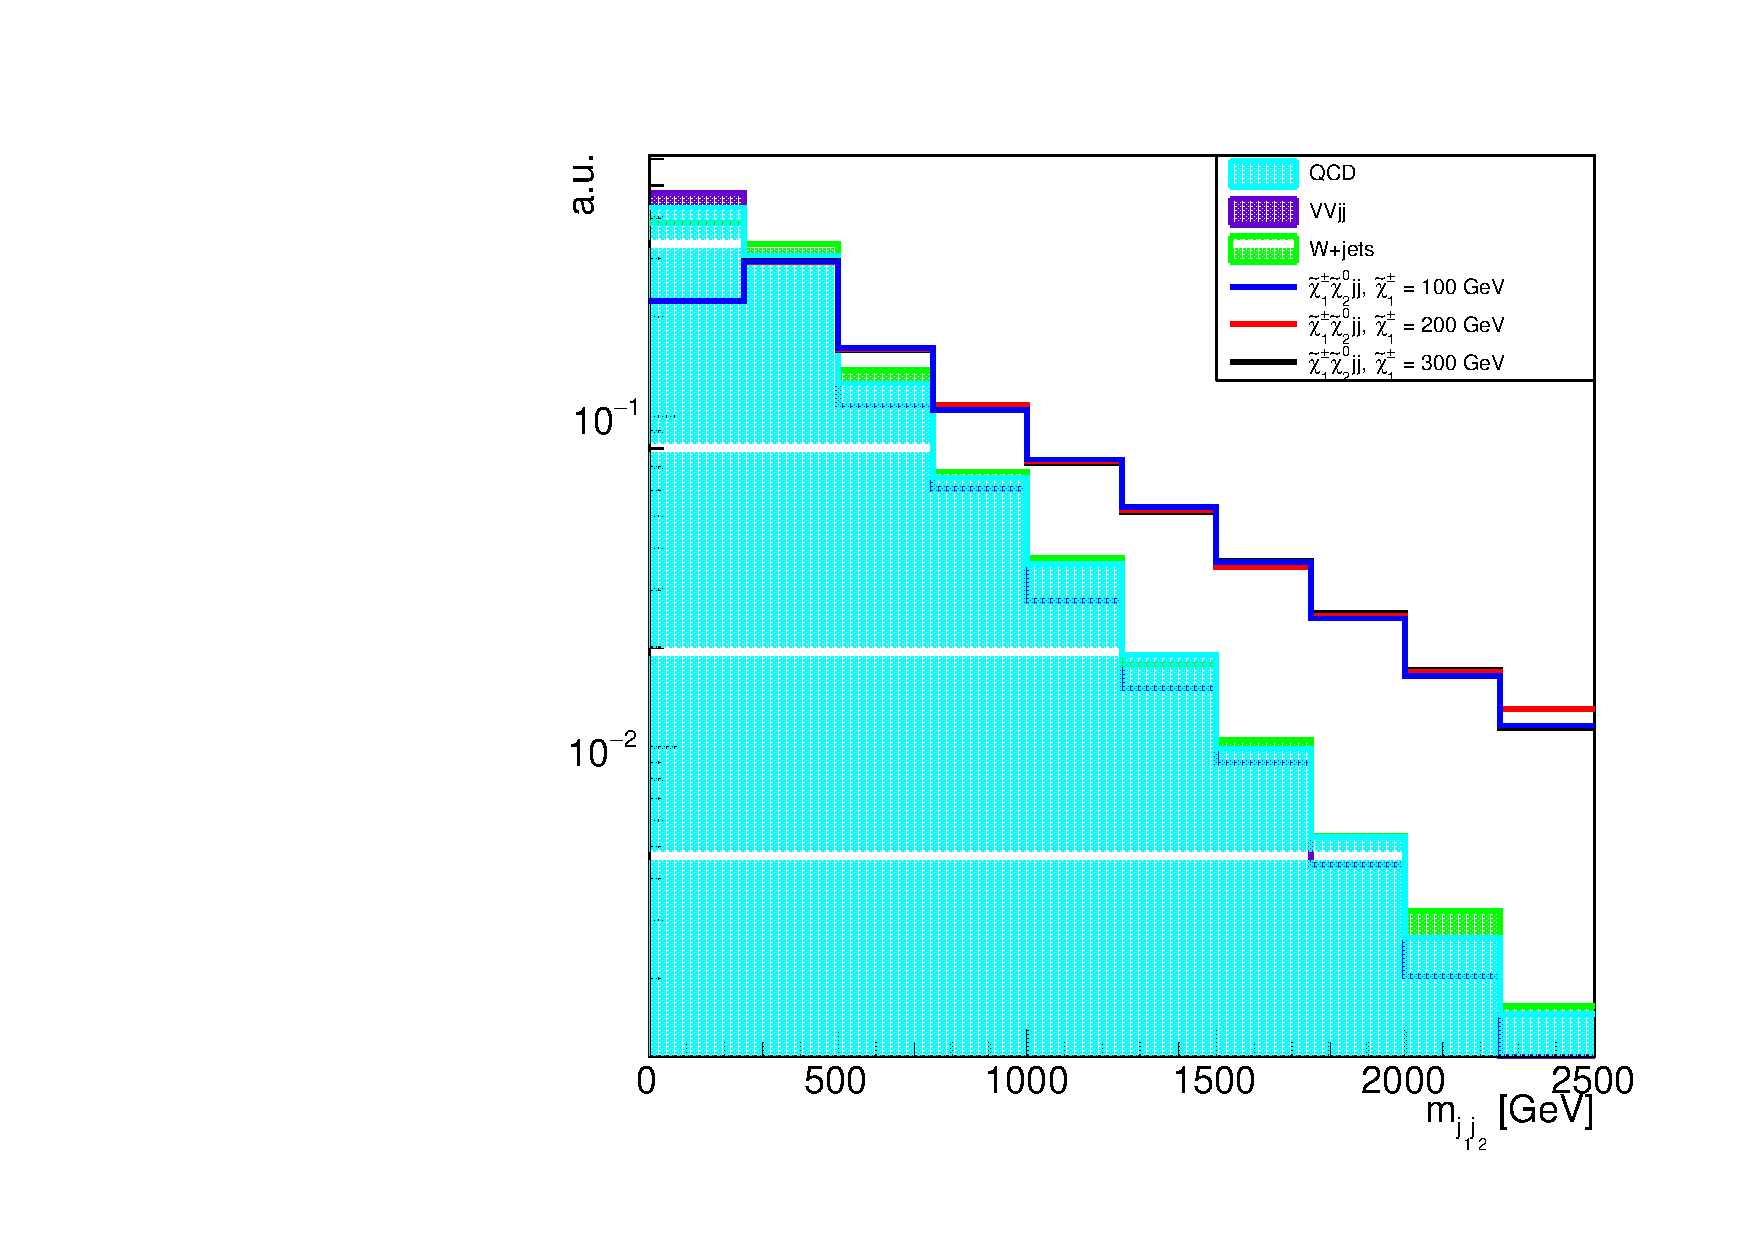
\includegraphics[width=0.48\textwidth]{analysis/pics/h_dijetinvariantmass_prospects13tev.pdf}
		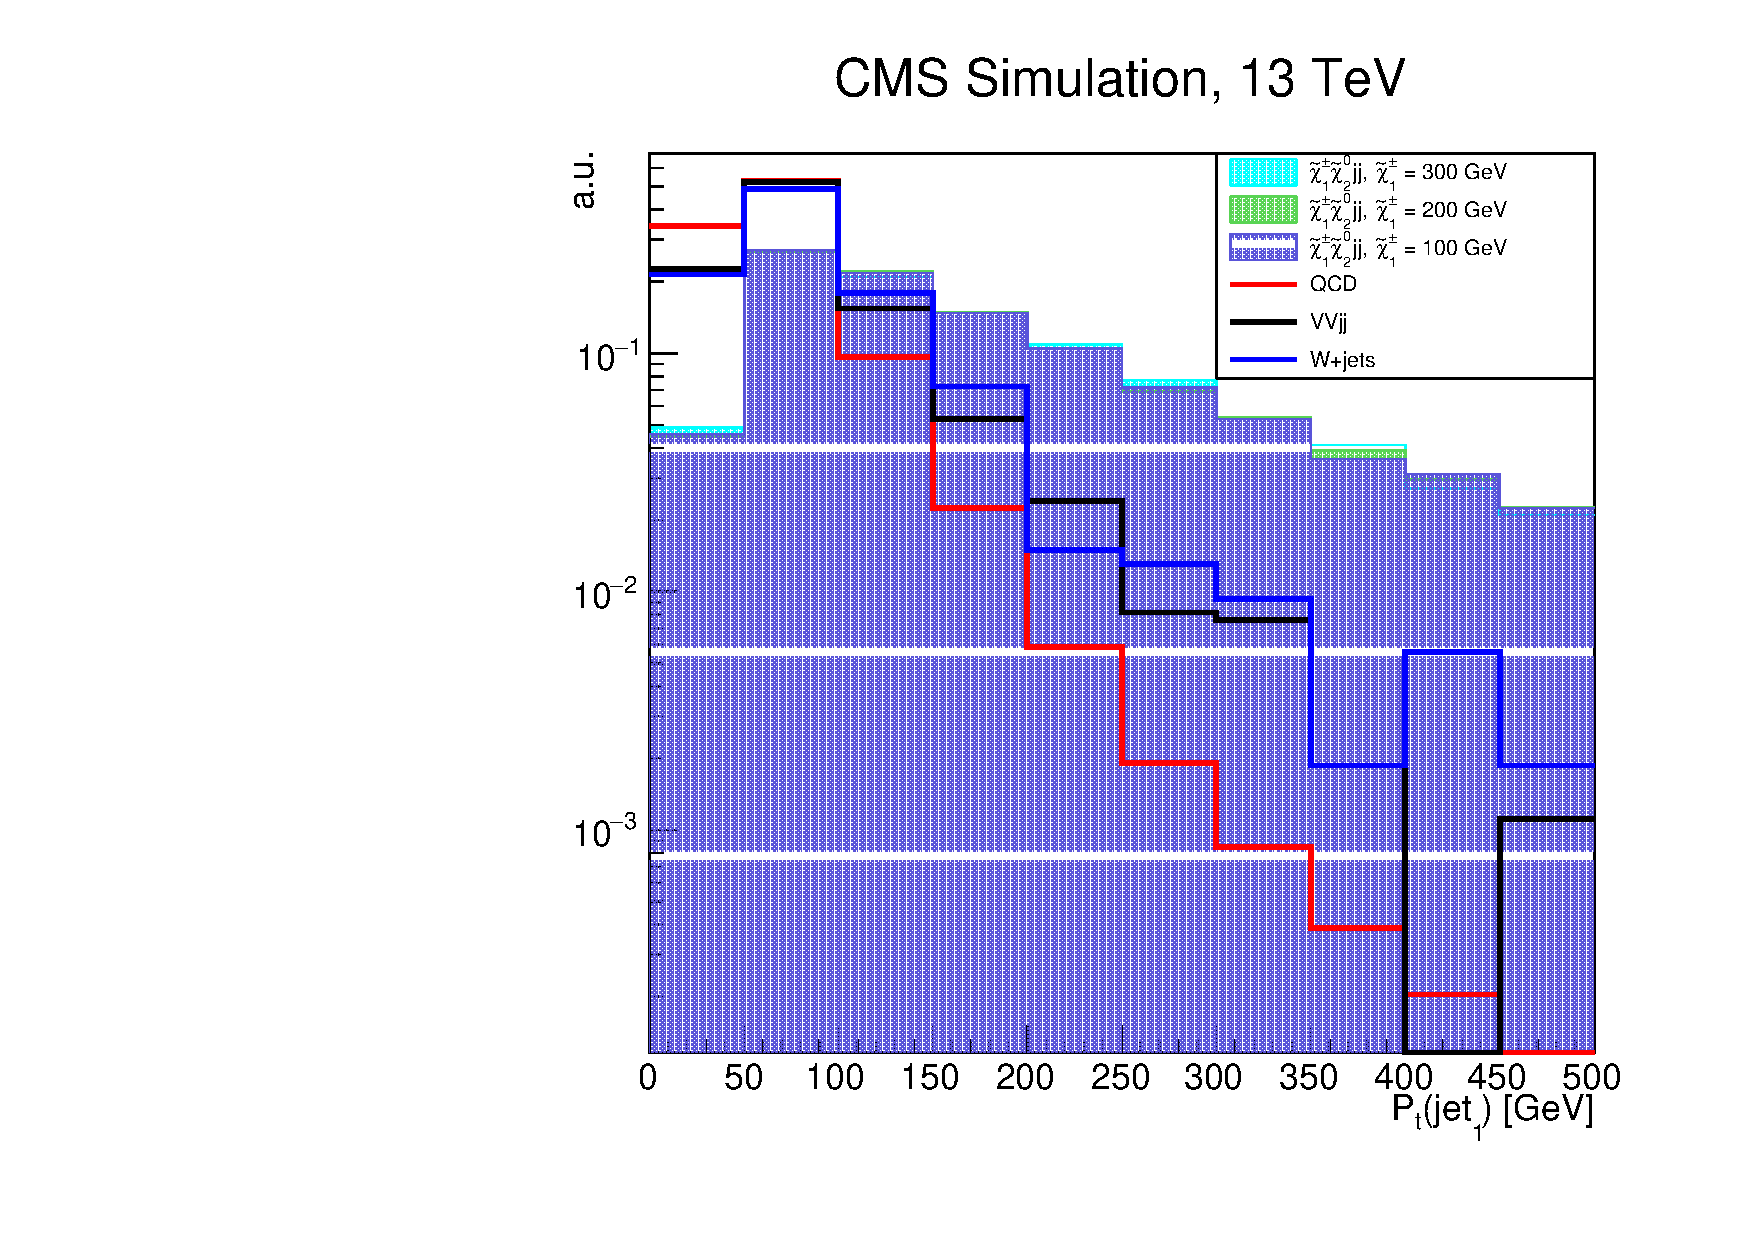
\includegraphics[width=0.48\textwidth]{analysis/pics/h_jet1pt_prospects13tev.pdf} 		
	\end{tabular}
	\caption{\ensuremath{m_{j_{1}j_{2}}} (left) and \pt of the leading jet (right) distributions normalized to arbitrary units for \charginopm \charginopm pair production by VBF processes, V+jets background, and VV background produced by VBF processes and QCD processes. The chosen signal benchmark point features \ensuremath{m_{\charginopm} = m_{\neutralinotwo} = 300\gev}, \ensuremath{m_{\charginopm} - m_{\tilde{\tau}} = 5\gev} and \ensuremath{m_{\neutralinoone} = 0\gev}.}
	\label{fig:VBF_mjj_ptj1}
\end{figure}


The remaining background contributions come from all the centrally produced particles. By considering an R-parity conserving model the decay of \charginopm and \neutralinotwo is the following

\begin{equation}
 \charginopm \longrightarrow \stau^{\pm} \nu \longrightarrow \tau^{\pm} \neutralinoone \nu
\end{equation}

\begin{equation}
\neutralinotwo \longrightarrow \stau^{\pm} \tau^{\mp} \longrightarrow \tau^{\pm} \tau^{\mp} \neutralinoone
\end{equation}

The \neutralinoone LSP travels through the detector undetected increasing \met. The processes that mimics signal are all the VV (where V may be wither W or Z) pairs produced via VBF where the bosons decays leptonically. A \met cut is effective in reducing this background as shown on Figure \ref{fig:VBF_met_pttau}. Moreover, requiring multiple $\tau$’s in the event further reduces background. The \pt of the \ensuremath{\tau} coming from the \charginopm and \neutralinotwo decays is strongly correlated to the mass difference between the \charginopm and the \neutralinoone LSP. In Figure \ref{fig:VBF_met_pttau}, the normalized distribution of the \pt of \ensuremath{\tau} is displayed for \ensuremath{m_{\charginopm} = m_{\neutralinotwo} = 300\gev}, \ensuremath{m_{\charginopm} - m_{\tilde{\tau}} = 5\gev} and \ensuremath{m_{\neutralinoone} = 0\gev}. For smaller \ensuremath{\Delta M}, the distribution peaks at lower \pt and the signal acceptance is less efficient.

\begin{figure}[tbh!]
	\centering
	\begin{tabular}{cc}
		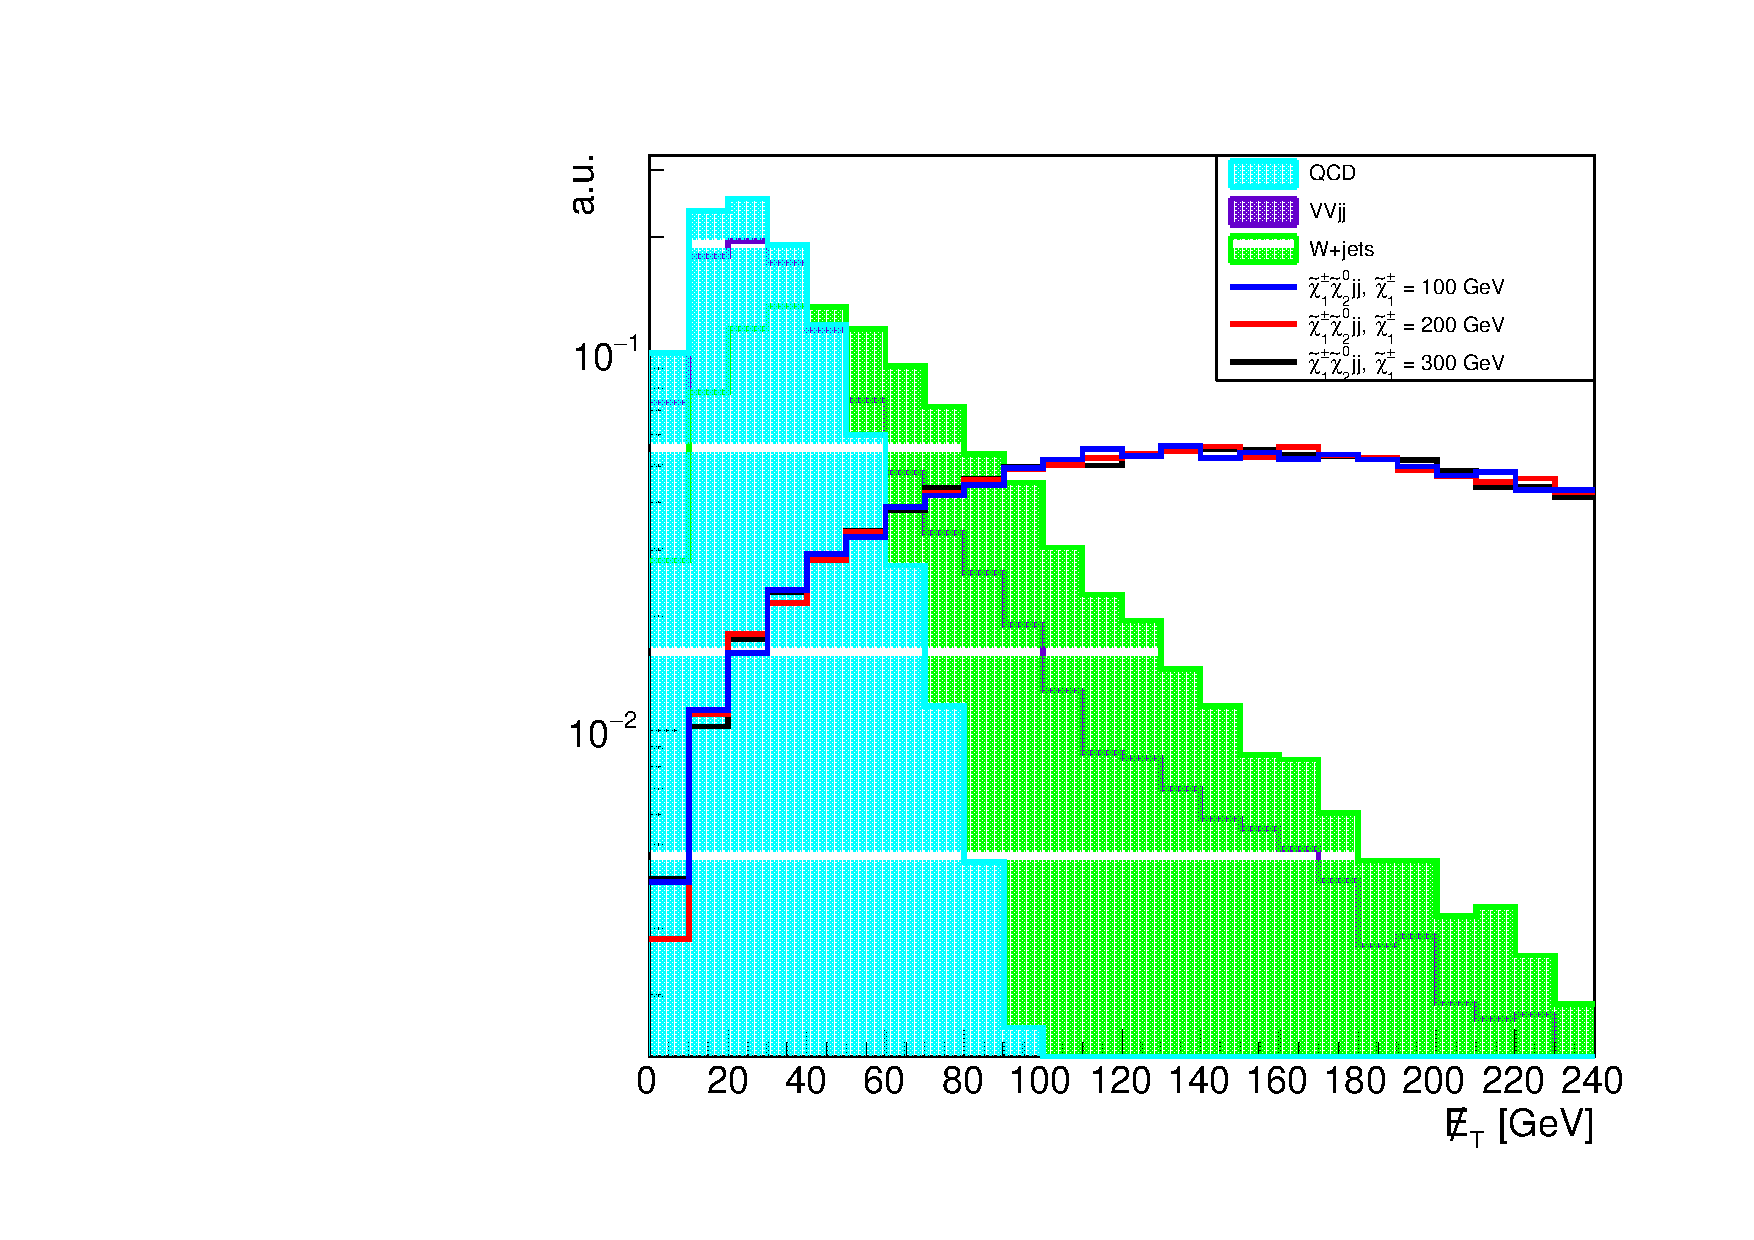
\includegraphics[width=0.48\textwidth]{analysis/pics/h_met_prospects13tev.pdf}
		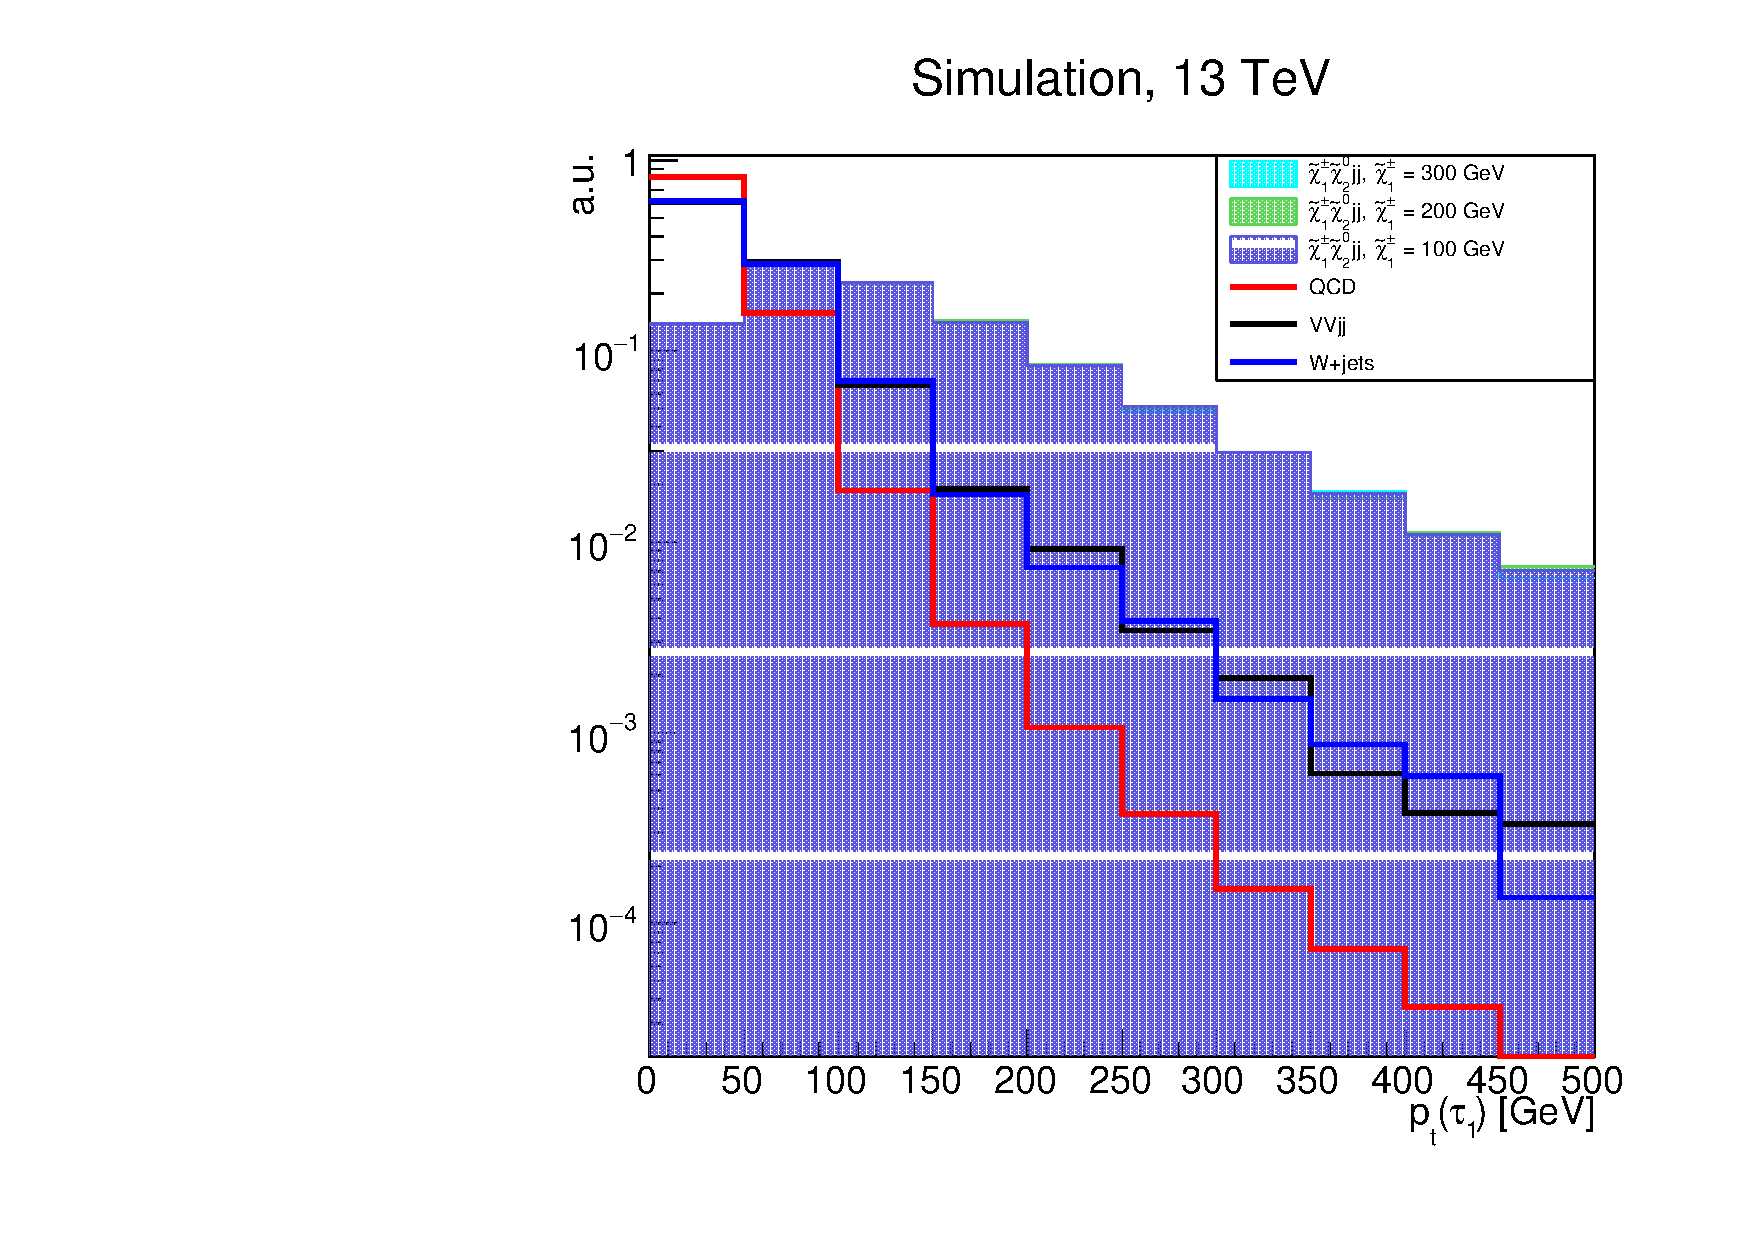
\includegraphics[width=0.48\textwidth]{analysis/pics/h_tau1pt_prospects13tev.pdf} 		
	\end{tabular}
	\caption{(left) \met and (right) leading \ensuremath{\tau} \pt distributions normalized to arbitrary units in \ensuremath{\geq 2j + 2\tau} final state for \charginopm \charginopm pair production by VBF processes, V+jets background, and VV background produced by VBF processes and QCD processes. The chosen signal benchmark point features \ensuremath{m_{\charginopm} = m_{\neutralinotwo} = 300\gev}, \ensuremath{m_{\charginopm} - m_{\tilde{\tau}} = 5\gev} and \ensuremath{m_{\neutralinoone} = 0\gev}.}
	\label{fig:VBF_met_pttau}
\end{figure}

